\documentclass[border=10pt]{standalone}
\usepackage{tikz}

\begin{document}
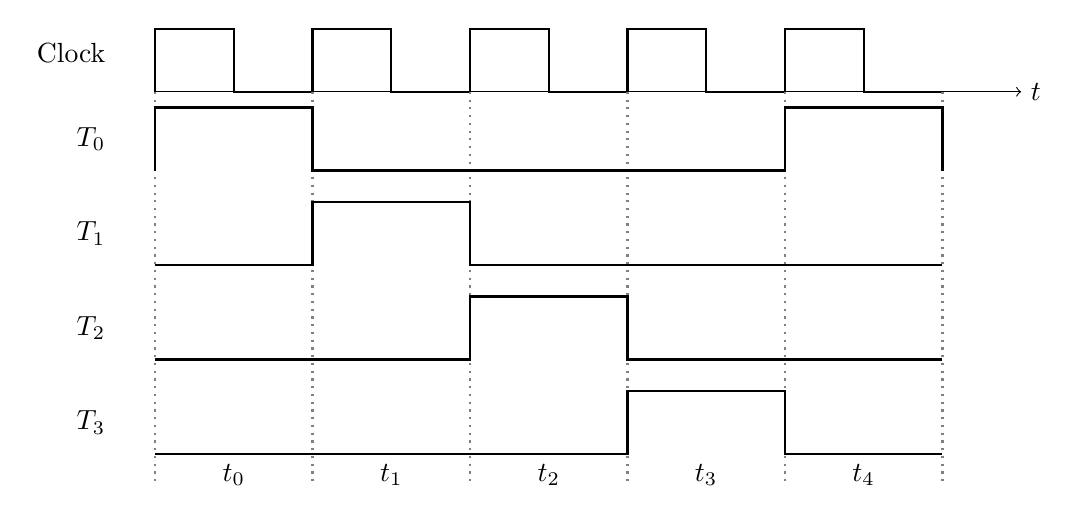
\begin{tikzpicture}[thick, scale=1.0]
  % Settings
  \def\h{0.8} % signal height
  
  % Clock
  \node[left] at (-0.5, 5.5) {Clock};
  % Draw Clock pulses
  % 5 periods shown (t0..t3, then t0 again)
  \foreach \i in {0, ..., 4} {
      \draw (\i*2, 5) -- ++(0, \h) -- ++(1, 0) -- ++(0, -\h) -- ++(1, 0);
      % Grid lines for clarity
      \draw[dotted, gray] (\i*2, 5.0) -- (\i*2, 0);
  }
  \draw[dotted, gray] (10, 5.0) -- (10, 0);
  \draw[->, thin] (0, 5) -- (11, 5) node[right] {$t$};
  
  % T0
  \node[left] at (-0.5, 4.4) {$T_0$};
  % High during t0 (0-2) and t4 (8-10)
  \draw (0, 4) -- ++(0, \h) -- ++(2, 0) -- ++(0, -\h) -- ++(6, 0) -- ++(0, \h) -- ++(2, 0) -- ++(0, -\h);
  
  % T1
  \node[left] at (-0.5, 3.2) {$T_1$};
  % High during t1 (2-4)
  \draw (0, 2.8) -- ++(2, 0) -- ++(0, \h) -- ++(2, 0) -- ++(0, -\h) -- ++(6, 0);
  
  % T2
  \node[left] at (-0.5, 2.0) {$T_2$};
  % High during t2 (4-6)
  \draw (0, 1.6) -- ++(4, 0) -- ++(0, \h) -- ++(2, 0) -- ++(0, -\h) -- ++(4, 0);
  
  % T3
  \node[left] at (-0.5, 0.8) {$T_3$};
  % High during t3 (6-8)
  \draw (0, 0.4) -- ++(6, 0) -- ++(0, \h) -- ++(2, 0) -- ++(0, -\h) -- ++(2, 0);

  % Cycle Labels
  \node[below] at (1, 0.4) {$t_0$};
  \node[below] at (3, 0.4) {$t_1$};
  \node[below] at (5, 0.4) {$t_2$};
  \node[below] at (7, 0.4) {$t_3$};
  \node[below] at (9, 0.4) {$t_4$};

\end{tikzpicture}
\end{document}
